% This file is a section fragment intended for inclusion with \input.
% The parent document should use XeLaTeX and load amsmath, amssymb,
% graphicx, and booktabs. Figure paths assume compilation from the
% project root directory.

\section{Numerical experiments}
\label{sec:maxwell-gpswf-numerics}

We present five tests of low-rank inversion with 3D Maxwell far-field data.
They examine the dimension of the ball GPSWF space, measurement noise, the
wavenumber, and the reconstruction basis. The forward and inverse stages are
kept separate in every experiment. A prescribed tensor contrast
$\mathbf{Q}(\mathbf{x})$ is first used to generate far-field measurements; the
inverse stage then uses only these measurements to recover Fourier samples and
reconstruct the contrast. Unless otherwise stated, the displayed quantity is
the real part of the $Q_{11}$ component on the plane $x_3=0$.

\subsection{Common numerical setting}
\label{subsec:maxwell-gpswf-setup}

The support of the unknown tensor contrast is assumed to be contained in the
unit ball
\[
    B=\{\mathbf{x}\in\mathbb{R}^3:|\mathbf{x}|<1\}.
\]
We use the general nonsymmetric complex reference tensor
\[
\mathbf{Q}_0=
\begin{pmatrix}
1+0.15\mathrm{i} & 0.35-0.20\mathrm{i} & -0.10+0.08\mathrm{i}\\
-0.28+0.12\mathrm{i} & -0.65+0.30\mathrm{i} & 0.22-0.18\mathrm{i}\\
0.16+0.04\mathrm{i} & -0.34+0.10\mathrm{i} & 0.75-0.35\mathrm{i}
\end{pmatrix}.
\]
Within each block, the tensor contrast is a complex scalar amplitude times
$\mathbf{Q}_0$. Reconstructions are evaluated on a $161\times161$ Cartesian
grid in $[-1,1]^2\times\{0\}$.

Let $\mathbf{d},\widehat{\mathbf{x}}\in\mathbb{S}^2$ denote the incident and
observation directions, respectively. We define
\begin{equation}
    \mathbf{p}=\frac{\mathbf{d}-\widehat{\mathbf{x}}}{2},
    \qquad C=2k,
    \label{eq:maxwell-fourier-node}
\end{equation}
and use the Fourier convention
\begin{equation}
    \widehat{\mathbf{Q}}(\mathbf{p})
    =\int_B \mathbf{Q}(\mathbf{y})
    \exp\!\left(-\mathrm{i}C\mathbf{p}\cdot\mathbf{y}\right)
    \mathrm{d}\mathbf{y}.
    \label{eq:maxwell-qhat}
\end{equation}
After removal of the common factor $k^2/(4\pi)$, the Born far-field channel is
written as
\begin{equation}
    \mathbf{g}
    (\widehat{\mathbf{x}},\mathbf{d},\mathbf{e};k)
    =\mathbf{P}(\widehat{\mathbf{x}})
    \widehat{\mathbf{Q}}(\mathbf{p})\mathbf{e},
    \qquad
    \mathbf{P}(\widehat{\mathbf{x}})
    =\mathbf{I}-\widehat{\mathbf{x}}\widehat{\mathbf{x}}^{\mathsf T},
    \qquad \mathbf{e}\perp\mathbf{d}.
    \label{eq:maxwell-born-channel}
\end{equation}

We expand the Fourier tensor in the full nine-dimensional tensor basis
$\{\mathbf{T}_r\}_{r=1}^{9}$ as
\[
    \widehat{\mathbf{Q}}(\mathbf{p})
    =\sum_{r=1}^{9}c_r(\mathbf{p})\mathbf{T}_r.
\]
Each direction pair is used with two mutually orthogonal incident
polarizations, while all three components of the far-field vector are retained.
Consequently, one direction pair provides six scalar equations. With $J=6$
direction configurations for each target Fourier node, the polarimetric system
has the form
\begin{equation}
    \mathbf{g}(\mathbf{p})
    =\mathbf{M}(\mathbf{p})\mathbf{c}(\mathbf{p}),
    \qquad
    \mathbf{M}(\mathbf{p})\in\mathbb{C}^{36\times9}.
    \label{eq:maxwell-polarimetric-system}
\end{equation}
The coefficient vector $\mathbf{c}(\mathbf{p})$ is recovered with the
Moore--Penrose inverse. The code requires every polarimetric matrix to have
column rank nine and records its smallest singular value and condition number.

Radial integration uses a Gauss--Jacobi rule adapted to the volume measure in
the unit ball, and angular integration uses a Lebedev rule on the unit sphere.
Finite incident and observation direction sets first
produce measurable Fourier nodes through~\eqref{eq:maxwell-fourier-node}. For
each target quadrature node, $J=6$ configurations are selected from a pool of
24 nearby candidates by prioritizing full rank, conditioning, and Fourier-node
distance. All formal experiments use 974 Lebedev incident directions and the
same 974 observation directions.

\subsection{Far-field data, noise, and spectral truncation}
\label{subsec:maxwell-gpswf-data}

Experiments 1--4 use Full VIE far-field data. For every incident direction and
polarization, the total field is obtained from
\begin{equation}
    \mathbf{E}(\mathbf{x})
    =\mathbf{E}^{\mathrm{i}}(\mathbf{x})
    +k^2\int_B \mathbf{G}_k(\mathbf{x},\mathbf{y})
    \mathbf{Q}(\mathbf{y})\mathbf{E}(\mathbf{y})\,\mathrm{d}\mathbf{y}.
    \label{eq:maxwell-full-vie}
\end{equation}
The far field generated from this total field is then passed to the same
Born-based inverse pipeline,
\begin{equation}
    \text{far-field data}
    \longrightarrow \widehat{\mathbf{Q}}(\mathbf{p})
    \longrightarrow Q_{11}(\mathbf{x}).
    \label{eq:maxwell-inversion-pipeline}
\end{equation}

Let $\mathbf{g}$ denote a noise-free far-field vector. Complex Gaussian
relative noise is added according to
\begin{equation}
    \mathbf{g}^{\delta}=\mathbf{g}+\boldsymbol{\eta},
    \qquad
    \|\boldsymbol{\eta}\|_2=\delta\|\mathbf{g}\|_2,
    \label{eq:maxwell-noise}
\end{equation}
where the real and imaginary parts of the unnormalized noise are independent
standard Gaussian vectors. The perturbation is added to the far-field channels
before polarimetric recovery, rather than to the recovered Fourier
coefficients.

The three-dimensional ball GPSWFs are denoted by
$\psi_{\ell,n,m}(\mathbf{x};C)$, where $\ell$ is the spherical-harmonic degree,
$m=-\ell,\ldots,\ell$ is its order, and $n$ is the radial index. The associated
prolate eigenvalue is $\alpha_{\ell,n}(C)$. The truncated reconstruction is
\begin{equation}
    Q_{11,N}(\mathbf{x})
    =\sum_{(\ell,n,m)\in\mathcal{I}_N}
    q_{\ell,n,m}\psi_{\ell,n,m}(\mathbf{x};C).
    \label{eq:maxwell-gpswf-reconstruction}
\end{equation}
Experiment 1 controls the low-rank dimension directly and retains every
$(\ell,n)$ multiplet as a complete set of $2\ell+1$ modes. Experiments 3 and 4
first impose
$|\alpha_{\ell,n}|>\varepsilon\max|\alpha|$ with $\varepsilon=0.2$, followed by
the cap
\begin{equation}
    N_{\mathrm{cap}}
    =\min\left\{\frac{C^2}{2},\frac{N_{\mathrm{quad}}}{6},512\right\},
    \label{eq:maxwell-mode-cap}
\end{equation}
while still retaining complete multiplets. The present implementation of
Experiment 2 uses the same prolate-eigenvalue threshold and then applies
$C^2/2$ as the total mode cap.

Table~\ref{tab:maxwell-experiment-summary} summarizes the five formal
experiments.
\begin{table}[htbp]
    \centering
    \caption{Main settings of the five Maxwell reconstruction experiments.}
    \label{tab:maxwell-experiment-summary}
    \begin{tabular}{lllll}
        \toprule
        Experiment & Quantity varied & Wavenumber $k$ & Noise $\delta$ & Data source\\
        \midrule
        1 & Low-rank dimension & $15$ & $0.2$ & Full VIE\\
        2 & Noise level & $15$ & $0,0.2,0.4$ & Full VIE\\
        3 & Frequency and resolution & $4,6,8,10,15,20$ & $0.2$ & Full VIE\\
        4 & Reconstruction method & $8,12,15$ & $0.2$ & Full VIE\\
        5 & Forward data source & $12$ & $0.2$ & Analytic Born/VIE--Born/Full VIE\\
        \bottomrule
    \end{tabular}
\end{table}

All figures below use the individual-scale outputs. Each panel therefore has
its own color limits and colorbar. These figures reveal weak structures and
shape changes, but their colors must not be used to compare absolute amplitudes
between panels.

\subsection{Effect of the low-rank dimension}
\label{subsec:maxwell-exp1}

Experiment 1 uses a cube centered at the origin with half-side length $0.4$.
Inside this cube the contrast is $\mathbf{Q}(\mathbf{x})=0.2\mathbf{Q}_0$.
We fix $k=15$, $C=30$, and $\delta=0.2$. The GPSWF discretization uses
$K=48$, $\ell_{\max}=12$, and seven radial modes for each $\ell$. The Full VIE
volume grid uses $n_{\mathrm{axis}}=23$. The retained
dimensions are arranged as
\[
\begin{array}{ccc}
1&5&21\\
35&57&71\\
135&237&496.
\end{array}
\]
Every value corresponds to a complete $(\ell,n)$ multiplet prefix. At low
dimension, only the location and coarse low-frequency structure can be
represented. Increasing the dimension introduces additional angular and radial
information and sharpens the reconstructed support. High-order modes are also
more sensitive to perturbations, so a larger dimension does not by itself imply
a smaller reconstruction error.

\begin{figure}[htbp]
    \centering
    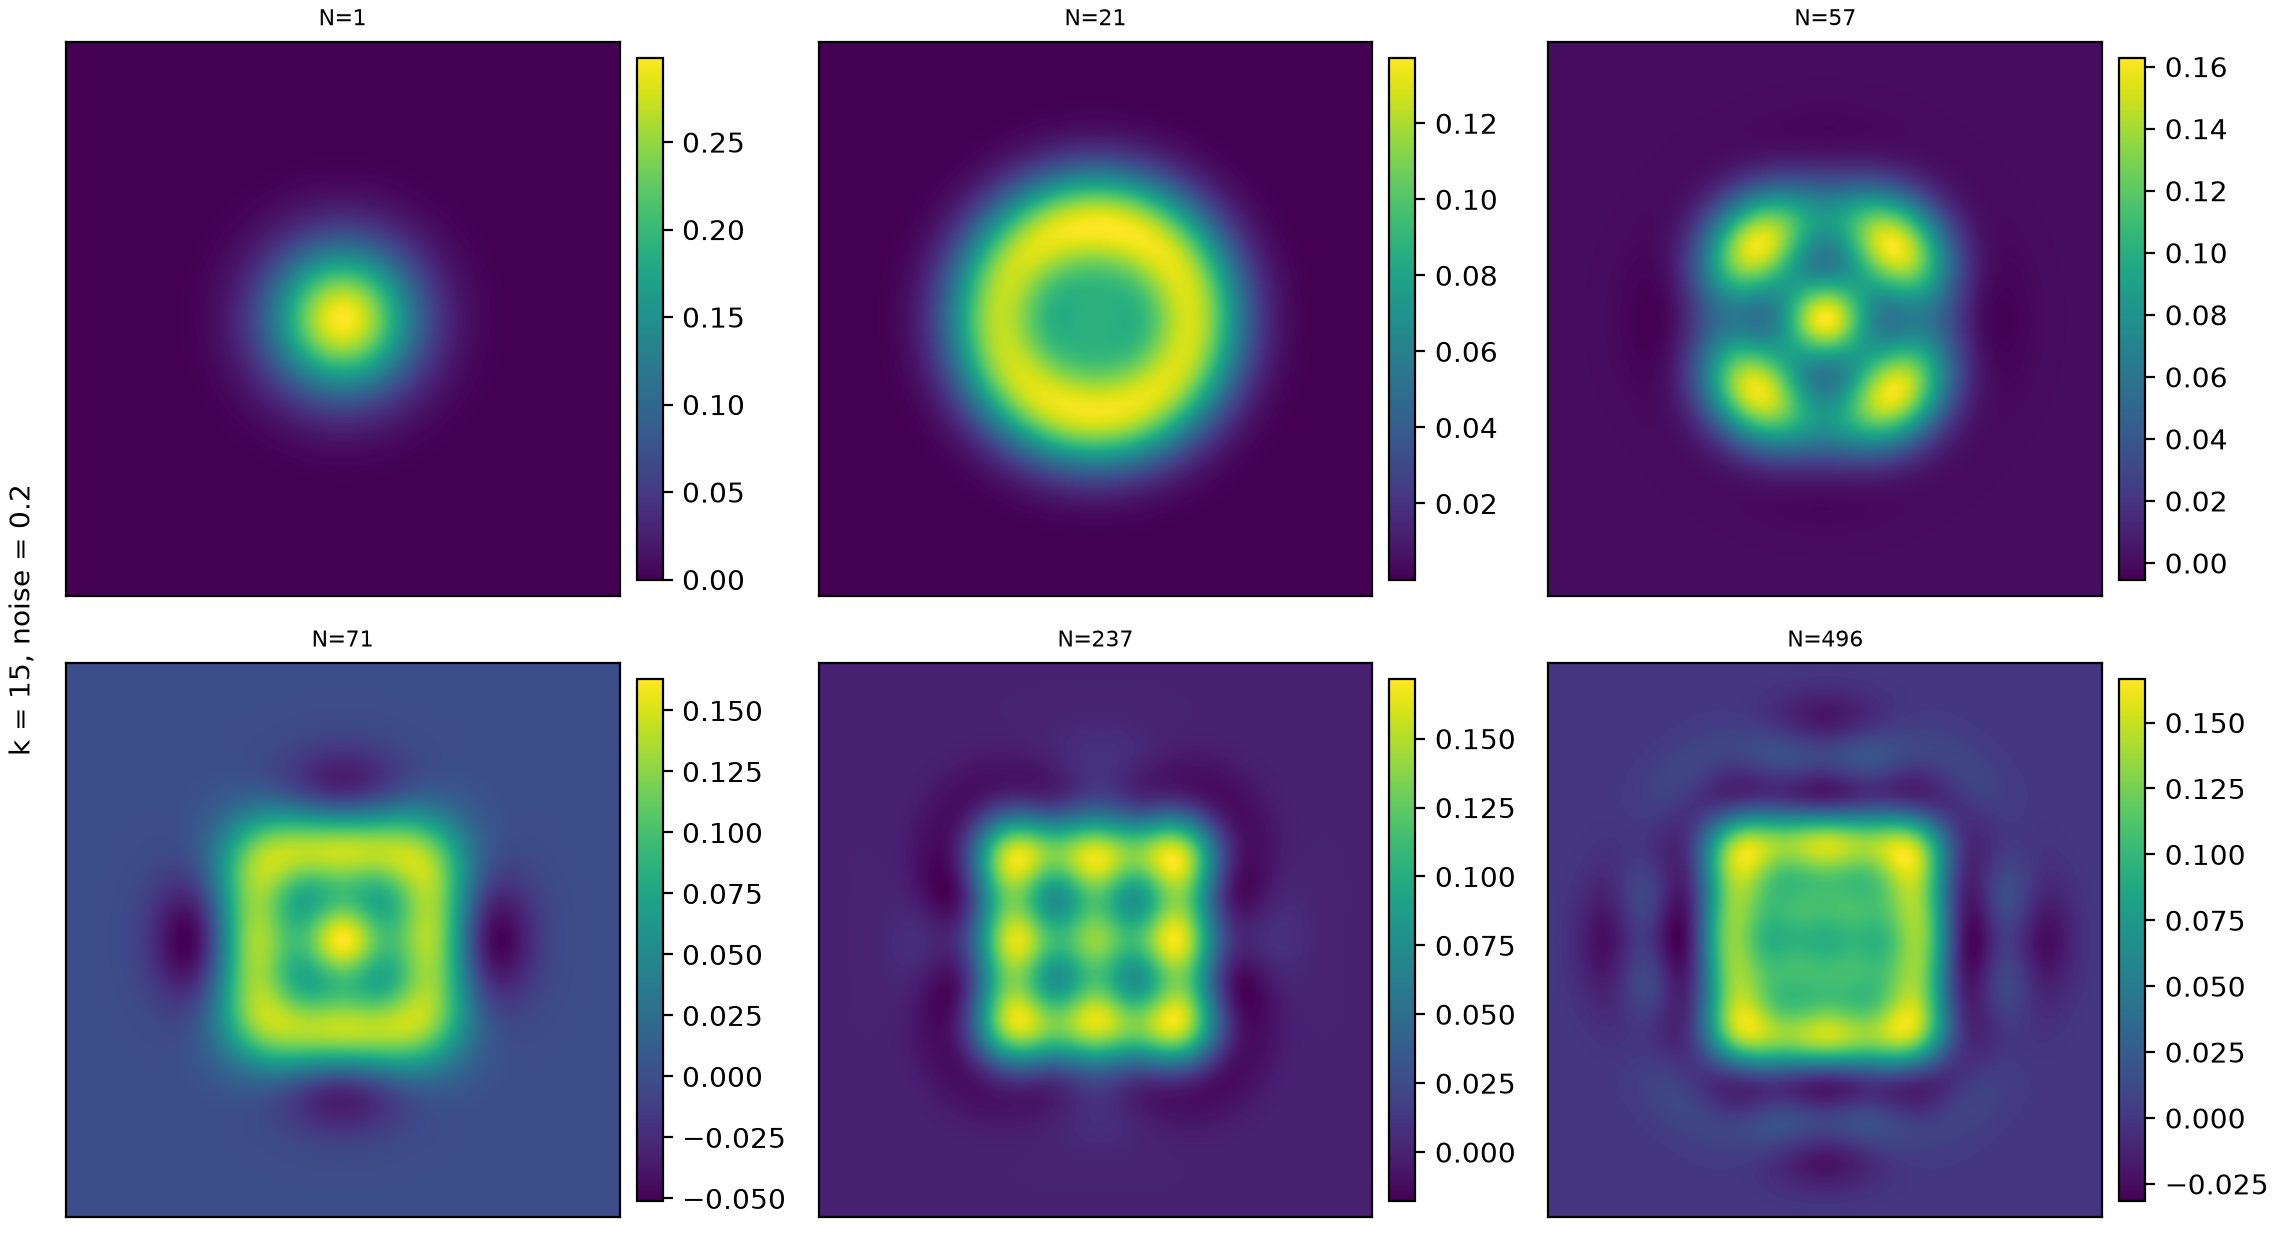
\includegraphics[width=0.88\textwidth]
    {outputs/exp1/exp1_dimension_individual_scale.png}
    \caption{Reconstruction of the $Q_{11}$ cross-section for increasing ball
    GPSWF dimensions. Here $k=15$ and $\delta=0.2$. Each panel uses its own
    color scale.}
    \label{fig:maxwell-exp1-dimension}
\end{figure}

To separate forward-model error from the noisy dimension experiment, we also
generate noiseless analytic Born and Full VIE far-field data using the same
incident directions, observation directions, polarizations, and target nodes.
Let $\mathbf{g}_{\mathrm{B}}$ and $\mathbf{g}_{\mathrm{F}}$ denote these two
far-field arrays. We record both
\begin{equation}
    e_{\mathrm{model}}
    =\frac{\|\mathbf{g}_{\mathrm{B}}-\mathbf{g}_{\mathrm{F}}\|_2}
    {\|\mathbf{g}_{\mathrm{F}}\|_2},
    \qquad
    e_{\mathrm{Born}}
    =\frac{\|\mathbf{g}_{\mathrm{F}}-\mathbf{g}_{\mathrm{B}}\|_2}
    {\|\mathbf{g}_{\mathrm{B}}\|_2},
\end{equation}
as well as the relative errors of the recovered full tensor
$\widehat{\mathbf{Q}}$ and its $(1,1)$ component. Radial bins in $|\mathbf{p}|$
show the RMS amplitude, relative error, and cross phase of
$\widehat{Q}_{11}$. No random noise is added to this diagnostic comparison.

\begin{figure}[htbp]
    \centering
    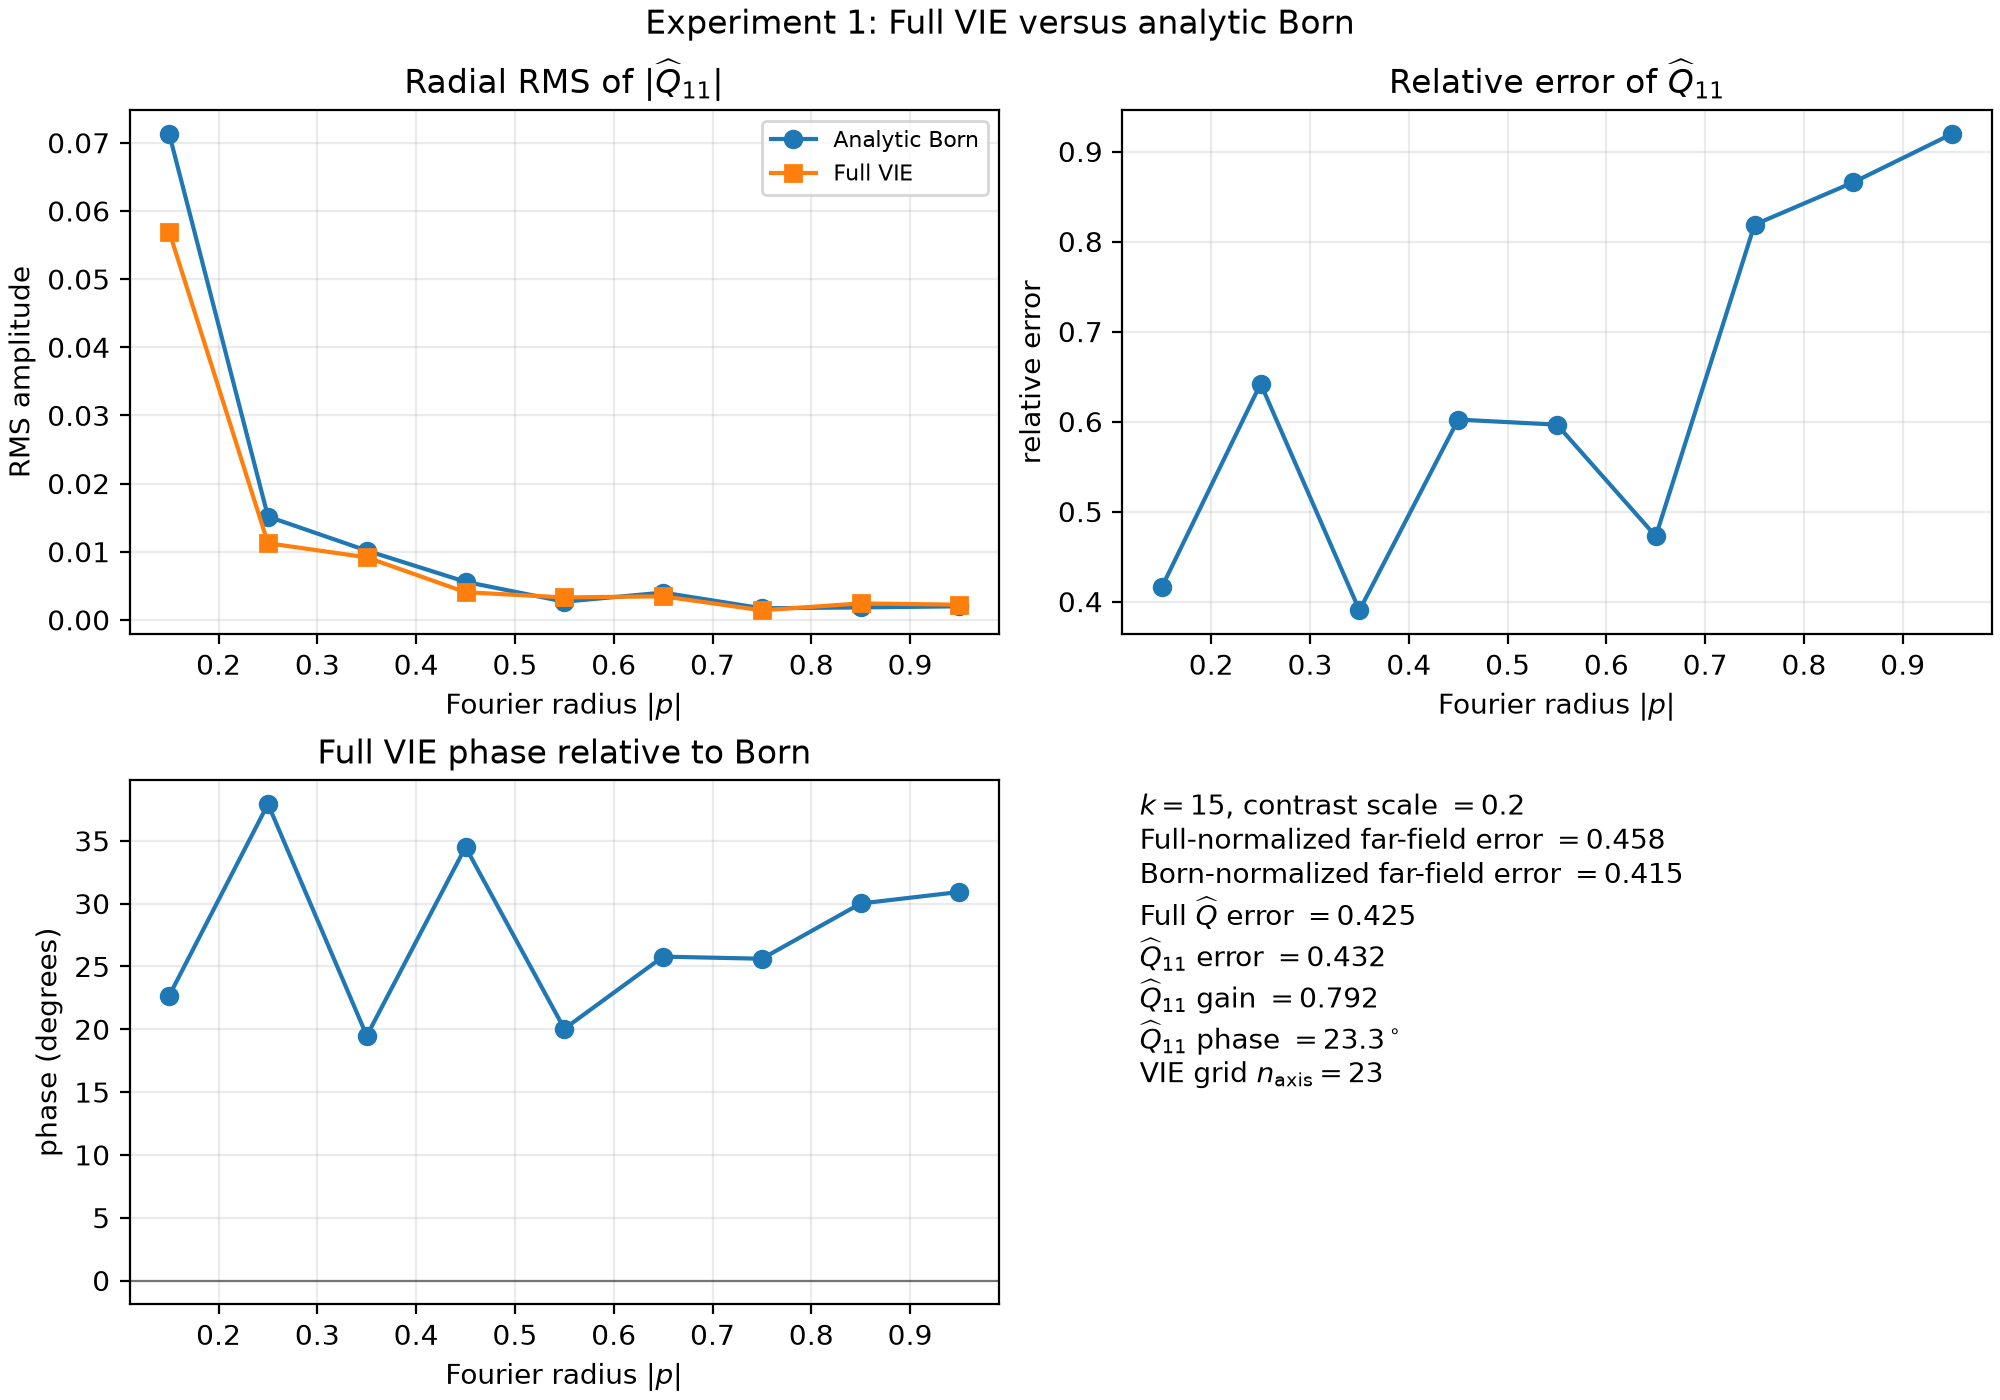
\includegraphics[width=0.88\textwidth]
    {outputs/exp1/exp1_full_vs_born_diagnostics.png}
    \caption{Noiseless Full VIE versus analytic Born diagnostics for
    Experiment 1. The curves expose the forward-model discrepancy separately
    from the noisy GPSWF dimension reconstructions.}
    \label{fig:maxwell-exp1-forward-diagnostics}
\end{figure}

\subsection{Robustness with respect to far-field noise}
\label{subsec:maxwell-exp2}

Experiment 2 fixes $k=15$ and uses the common three-block geometry with minimum
boundary separation $0.20$ and different complex amplitudes. Relative noise
levels $\delta=0,0.2,0.4$ are added directly
to one common Full VIE far-field data set, computed with
$n_{\mathrm{axis}}=19$. The direction sets, quadrature nodes, polarimetric
configurations, and GPSWF truncation are identical in all three cases, so the
only varying parameter is the noise level. The principal diagnostics are the
mean target amplitude, the 95th percentile of the background amplitude, the
polarimetric condition number, and the norm of the reconstruction coefficients.

\begin{figure}[htbp]
    \centering
    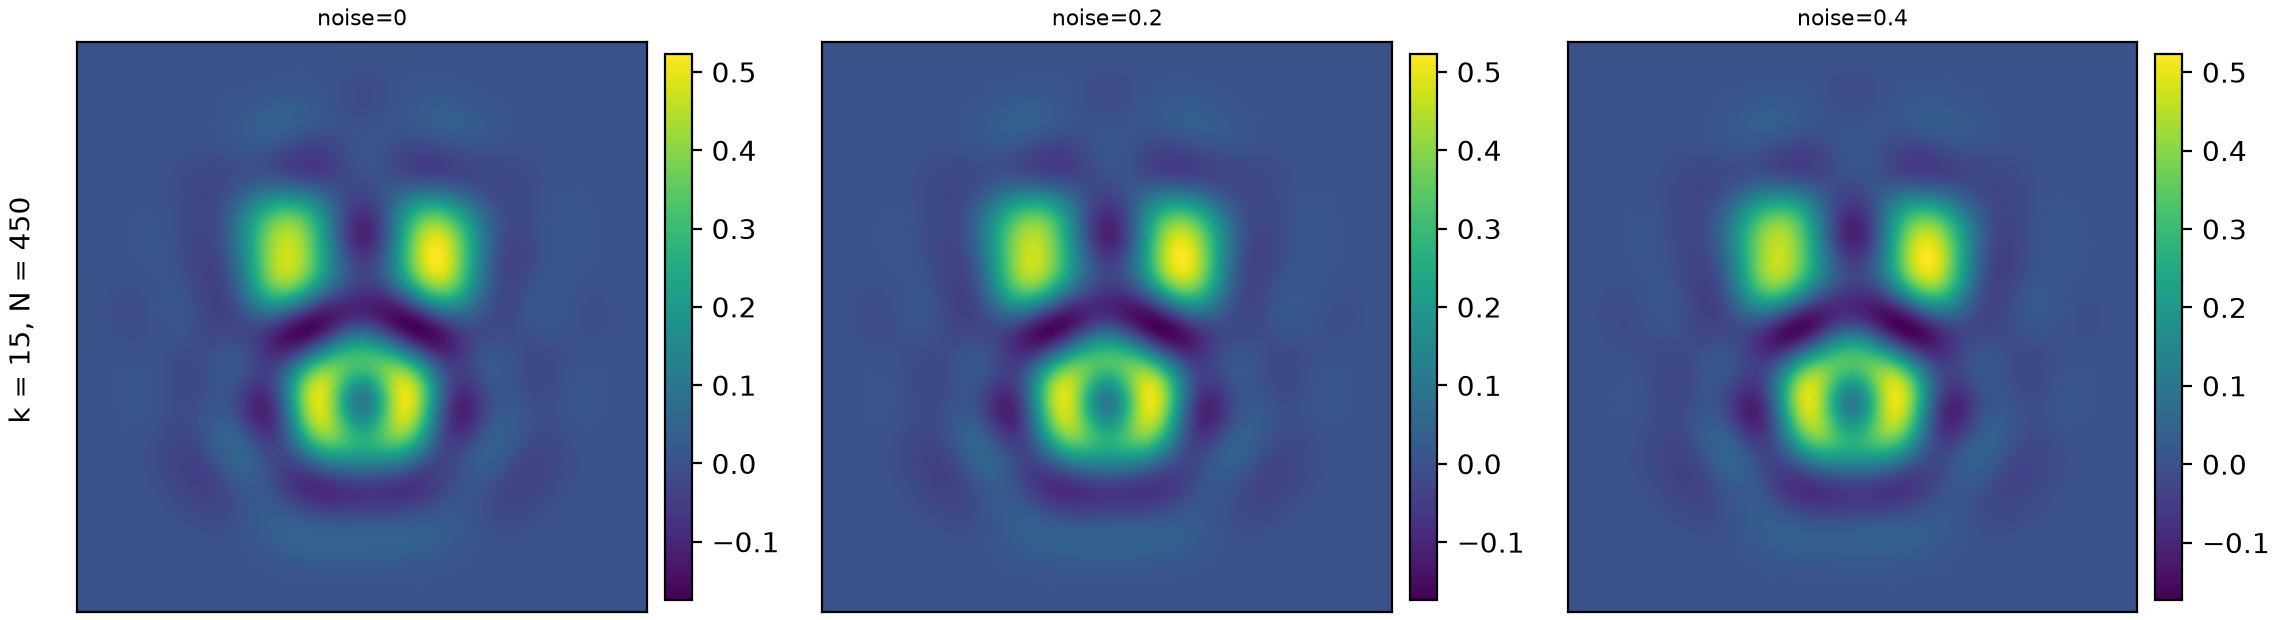
\includegraphics[width=0.96\textwidth]
    {outputs/exp2/exp2_noise_individual_scale.png}
    \caption{Reconstruction of the gap-$0.20$ three-block phantom for relative
    far-field noise levels $\delta=0,0.2,0.4$. Here $k=15$. Each panel uses its
    own color scale.}
    \label{fig:maxwell-exp2-noise}
\end{figure}

\subsection{Wavenumber and resolution}
\label{subsec:maxwell-exp3}

Experiment 3 uses three rectangular blocks whose minimum boundary separation
is $0.20$, and considers $k=4,6,8,10,15,20$. Full VIE generates the far-field
data at every frequency. The relative noise level is fixed
at $\delta=0.2$, and all six cases use the same 974 incident and observation
directions. The GPSWF and Full VIE parameters are listed
in Table~\ref{tab:maxwell-exp3-parameters}.

\begin{table}[htbp]
    \centering
    \caption{Ball GPSWF and Full VIE discretization parameters in Experiment 3.}
    \label{tab:maxwell-exp3-parameters}
    \begin{tabular}{rrrrrrrr}
        \toprule
        $k$ & $C$ & $K$ & $\ell_{\max}$ & $n_{\ell}$
        & $n_r$ & $n_{\mathrm{ang}}$ & $n_{\mathrm{axis}}$\\
        \midrule
        4  & 8  & 20 & 4  & 2 & 6  & 74  & 11\\
        6  & 12 & 26 & 5  & 3 & 8  & 110 & 11\\
        8  & 16 & 32 & 7  & 3 & 10 & 146 & 11\\
        10 & 20 & 40 & 8  & 5 & 12 & 194 & 12\\
        15 & 30 & 64 & 12 & 6 & 20 & 302 & 18\\
        20 & 40 & 80 & 14 & 7 & 28 & 434 & 19\\
        \bottomrule
    \end{tabular}
\end{table}

For a wavenumber $k$, the half wavelength is $\pi/k$. If objects separated by
less than $\pi/k$ remain distinguishable, the result is super-resolved relative
to that single frequency. Increasing $k$ enlarges the accessible Fourier band
and the effective rank of the continuous operator. However, the number of
modes that can be carried stably by the discrete system is also limited by the
quadrature density, mock-node mismatch, polarimetric conditioning, and noise.
The experiment therefore records both the retained dimension and discrete
stability diagnostics instead of assuming that every additional high-frequency
mode is useful.

\begin{figure}[htbp]
    \centering
    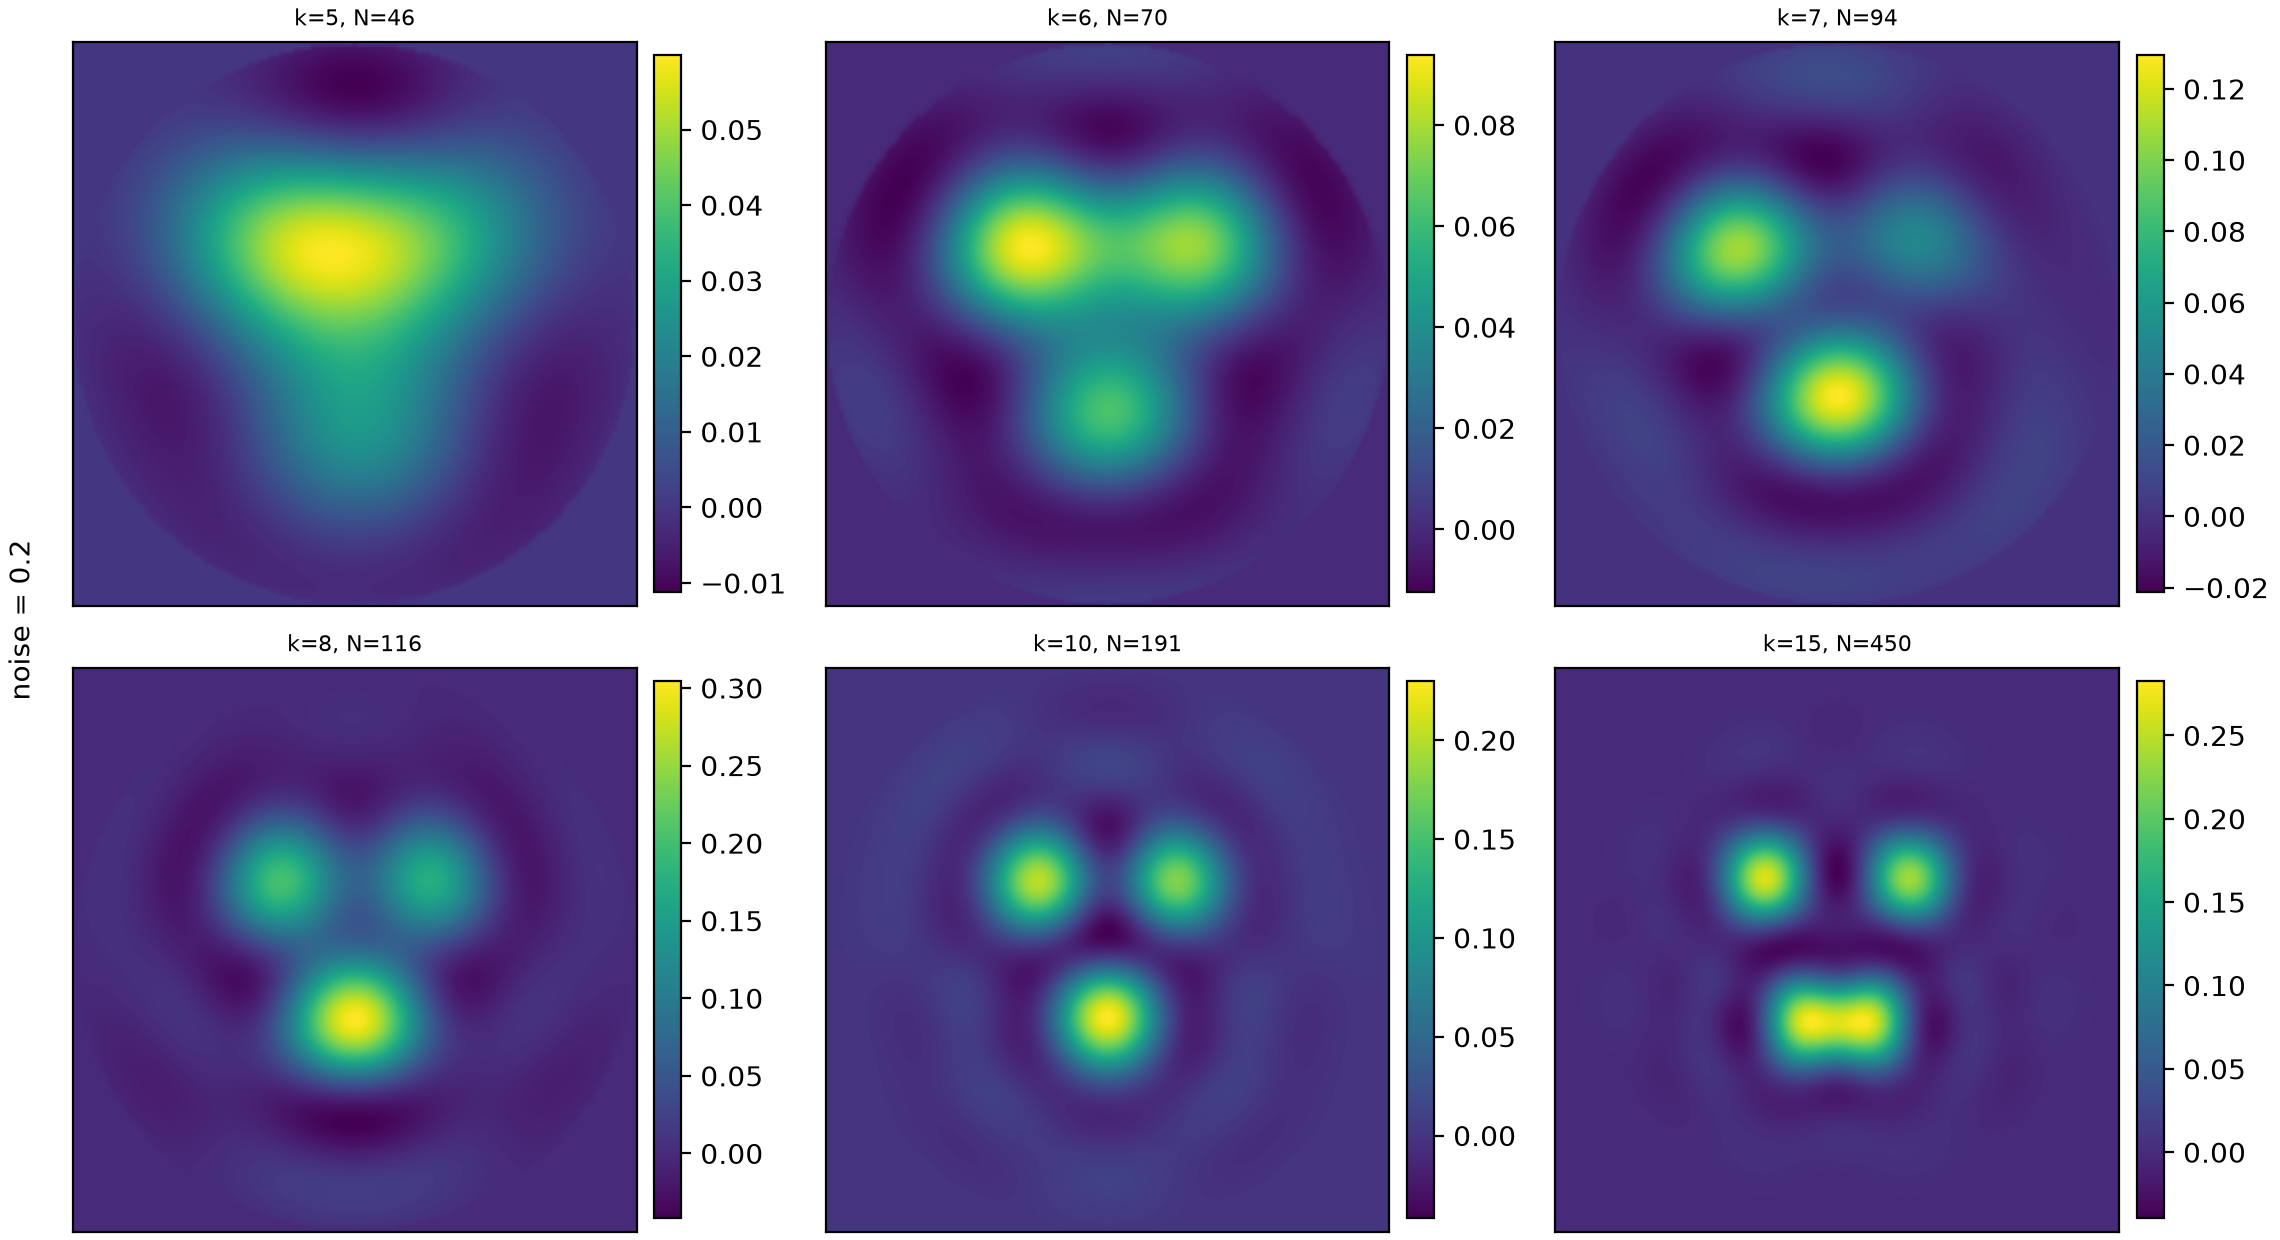
\includegraphics[width=0.72\textwidth]
    {outputs/exp3/exp3_frequency_individual_scale.png}
    \caption{Reconstruction of three closely spaced blocks for different
    wavenumbers. The minimum boundary separation is $0.20$ and
    $\delta=0.2$. Each panel uses its own color scale.}
    \label{fig:maxwell-exp3-frequency}
\end{figure}

The same recovered $\widehat{Q}_{11}(\mathbf{p})$ is also passed to the
normalized DSM indicator
\begin{equation}
    I_{\mathrm{DSM}}(\mathbf{z})
    =\left|\sum_s w_s\widehat{Q}_{11}(\mathbf{p}_s)
    \exp(\mathrm{i}C\mathbf{p}_s\cdot\mathbf{z})\right|.
\end{equation}
Thus, the GPSWF and DSM frequency figures differ only in the final imaging
operator, not in the Full VIE data, noise, or polarimetric recovery.

\begin{figure}[htbp]
    \centering
    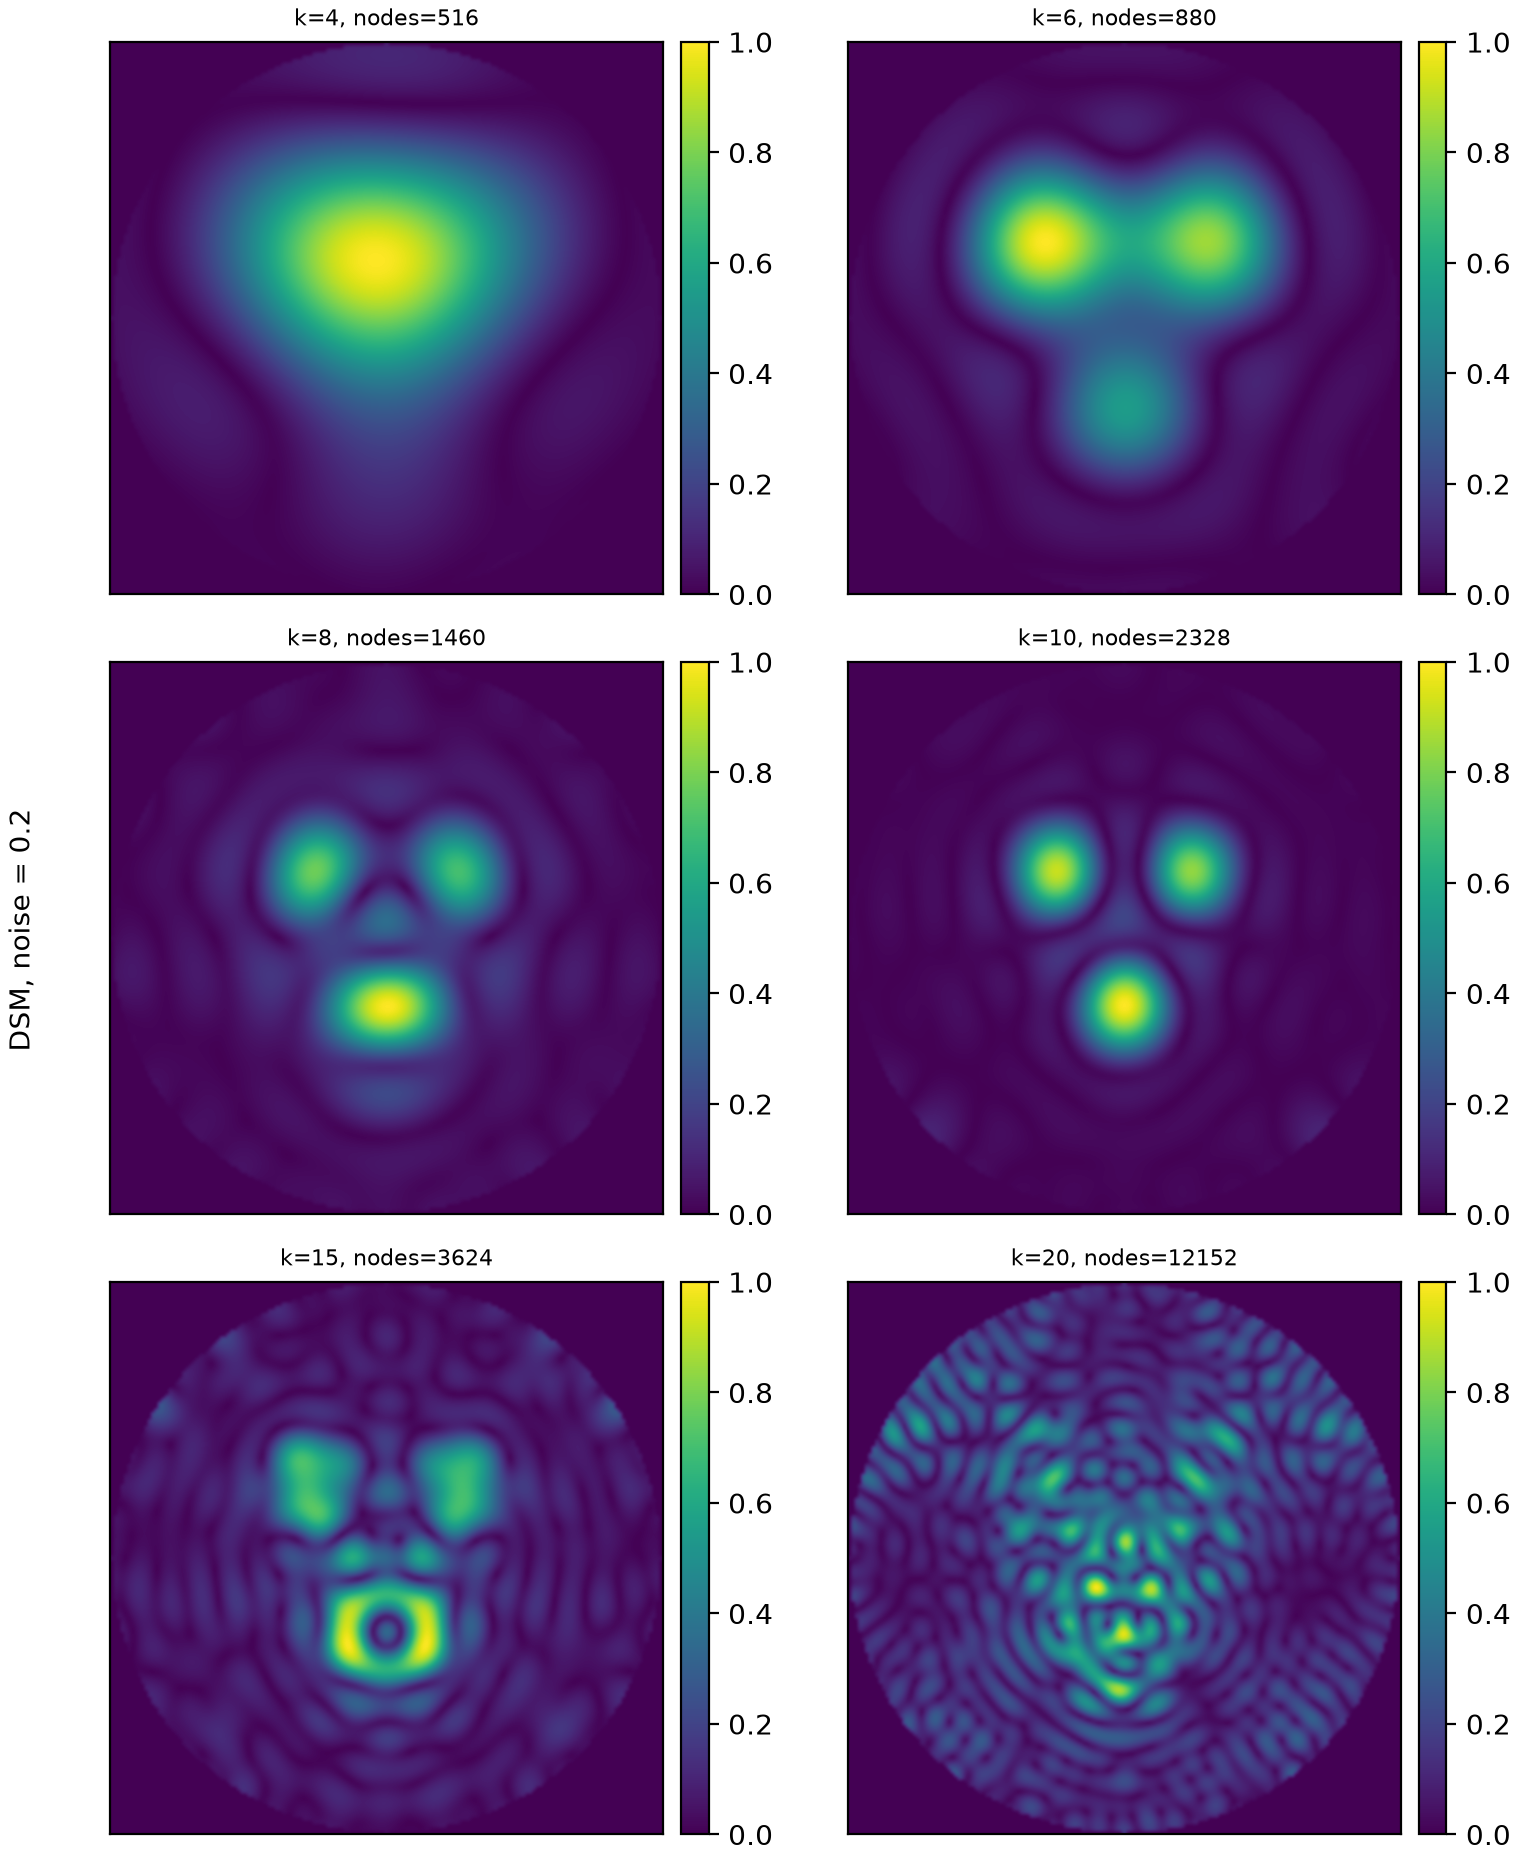
\includegraphics[width=0.72\textwidth]
    {outputs/exp3/exp3_frequency_dsm.png}
    \caption{Normalized DSM indicators from the same Full VIE data used in
    Figure~\ref{fig:maxwell-exp3-frequency}.}
    \label{fig:maxwell-exp3-dsm}
\end{figure}

\subsection{Comparison of reconstruction methods}
\label{subsec:maxwell-exp4}

Experiment 4 uses the same gap-$0.20$ three-block geometry and fixes the same
Full VIE far-field data, polarimetrically recovered
$\widehat{Q}_{11}(\mathbf{p})$, and target quadrature nodes, and compares ball
GPSWFs, a cube Fourier basis, a spherical-harmonic Bessel basis, and the direct
sampling method (DSM). We use $k=8,12,15$ and $\delta=0.2$. Consequently, the
differences between columns arise from the representation and regularization
used to map Fourier data into physical space, rather than from different
forward data or polarimetric recovery procedures.

\begin{table}[htbp]
    \centering
    \caption{GPSWF discretization parameters in Experiment 4.}
    \label{tab:maxwell-exp4-parameters}
    \begin{tabular}{rrrrrrr}
        \toprule
        $k$ & $C$ & $K$ & $\ell_{\max}$ & $n_{\ell}$
        & $n_r$ & $n_{\mathrm{ang}}$\\
        \midrule
        8  & 16 & 28 & 7  & 3 & 8  & 86\\
        12 & 24 & 40 & 9  & 5 & 10 & 170\\
        15 & 30 & 48 & 12 & 6 & 12 & 230\\
        \bottomrule
    \end{tabular}
\end{table}

The GPSWF branch uses the stable cap~\eqref{eq:maxwell-mode-cap}. The mode caps
for the cube Fourier and spherical Bessel bases are set to 1.2 times the actual
GPSWF dimension and are limited to at most 512 modes. Their weighted
least-squares cutoff is $10^{-8}$. DSM does not solve for expansion
coefficients; instead, it correlates the recovered Fourier data with
sampling-point test functions and normalizes the resulting indicator. A fair
comparison must consider object separation, background artifacts, and retained
mode counts in addition to the independently scaled images.

\begin{figure}[htbp]
    \centering
    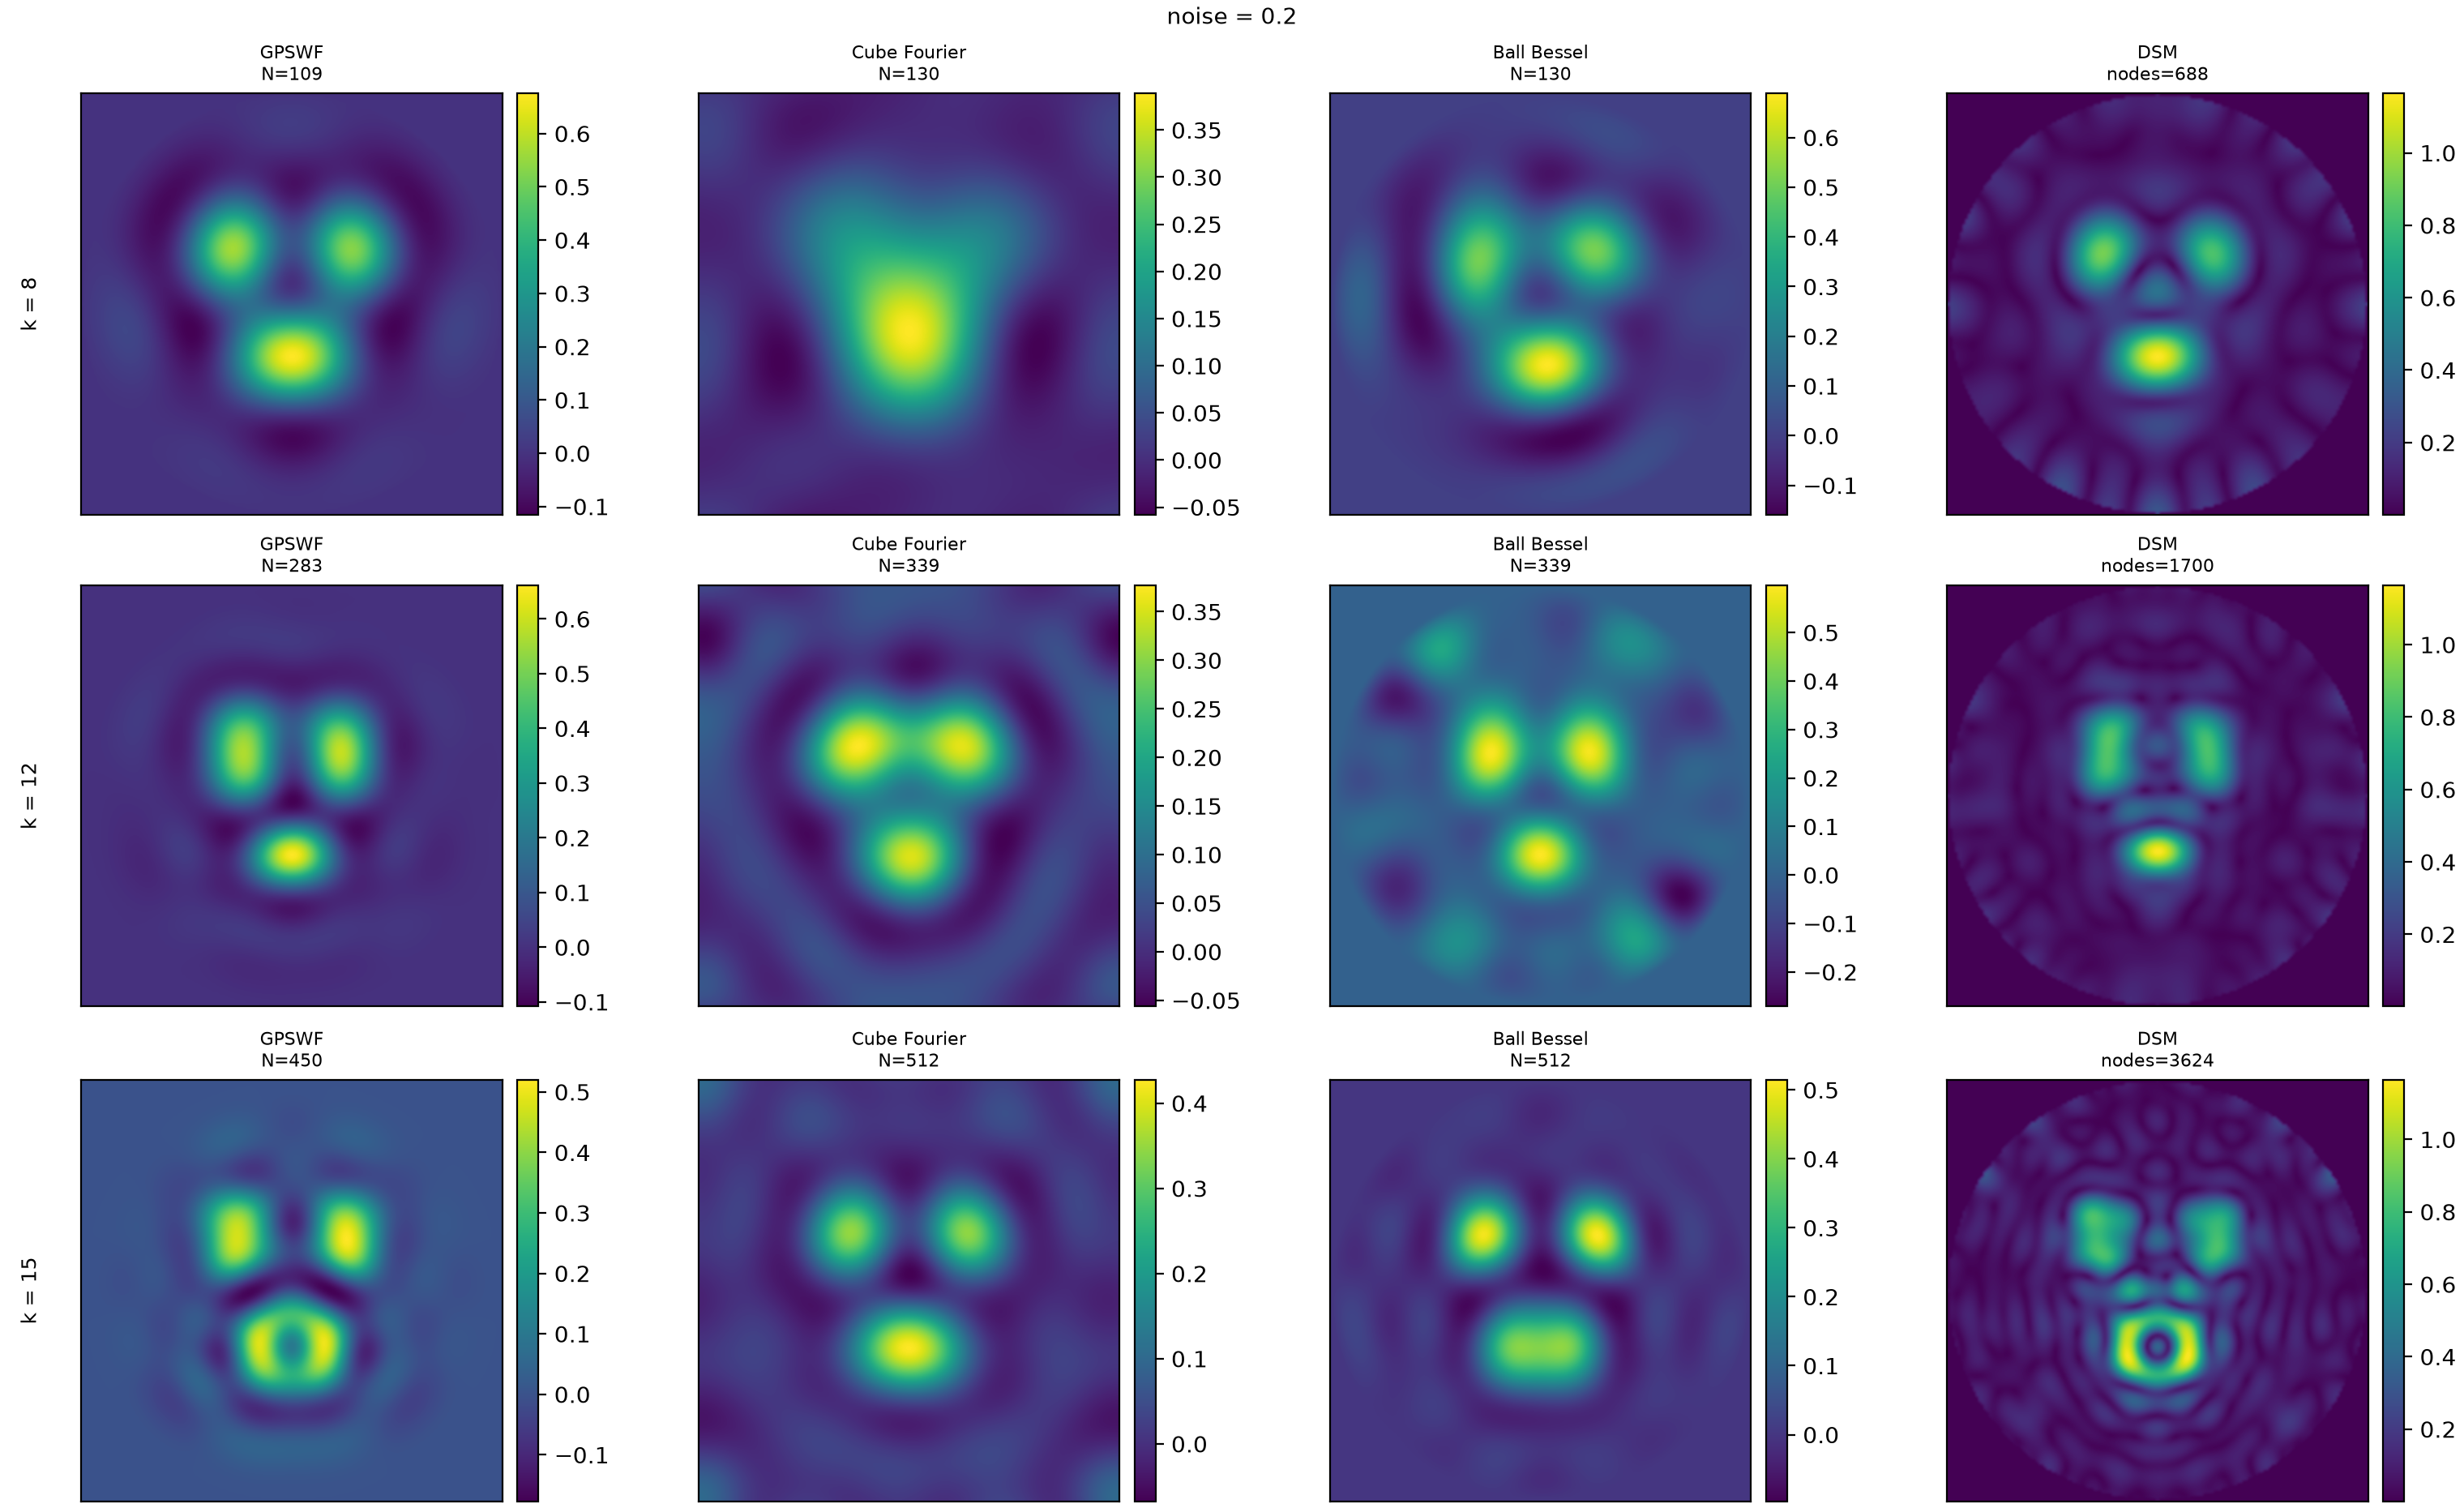
\includegraphics[width=\textwidth]
    {outputs/exp4/exp4_basis_individual_scale.png}
    \caption{Comparison of GPSWF, cube Fourier, spherical Bessel, and DSM
    reconstructions for different wavenumbers. Here $\delta=0.2$. Every panel
    has an independent color scale.}
    \label{fig:maxwell-exp4-bases}
\end{figure}

\subsection{Comparison of forward data sources}
\label{subsec:maxwell-exp5}

Experiment 5 fixes $k=12$, $C=24$, and $\delta=0.2$, and applies the four
reconstruction methods from Experiment 4 to three forward data sources. The
analytic Born source evaluates the block Fourier integrals at the actual mock
measurement nodes. The discrete VIE--Born source replaces those integrals by
voxel quadrature while setting the total field equal to the incident field.
The Full VIE source solves~\eqref{eq:maxwell-full-vie} and then evaluates the
far-field integral with the computed total field. Hence
the three rows respectively expose the continuous-block analytic Born formula,
voxel quadrature error within the Born model, and the combined effects of VIE
discretization and multiple scattering.

All rows use the same gap-$0.20$ three-block phantom, 974 incident directions,
974 observation directions, target quadrature nodes, mock configurations,
polarimetric matrices, and modal truncations. They also use the same standard
complex Gaussian noise realization, normalized separately to relative level
$0.2$ for each far-field data set. Thus, every row follows
\begin{equation}
    \text{far-field data}
    \longrightarrow \widehat{\mathbf{Q}}^{\delta}(\mathbf{p})
    \longrightarrow Q_{11}^{\delta}(\mathbf{x}),
    \label{eq:maxwell-exp5-pipeline}
\end{equation}
and no row sends an exact Fourier transform of the phantom directly to a
reconstruction method.

The formal Full VIE discretization uses $n_{\mathrm{axis}}=14$, giving 1472
voxel nodes and 4416 electric-field unknowns. The system matrix is assembled
and factorized once. The two incident polarizations are solved as multiple
right-hand sides, and the total fields are reused for all observation
directions associated with the same incident direction. This reuse changes
only the computational organization, not the VIE model or far-field formula.

\begin{figure}[htbp]
    \centering
    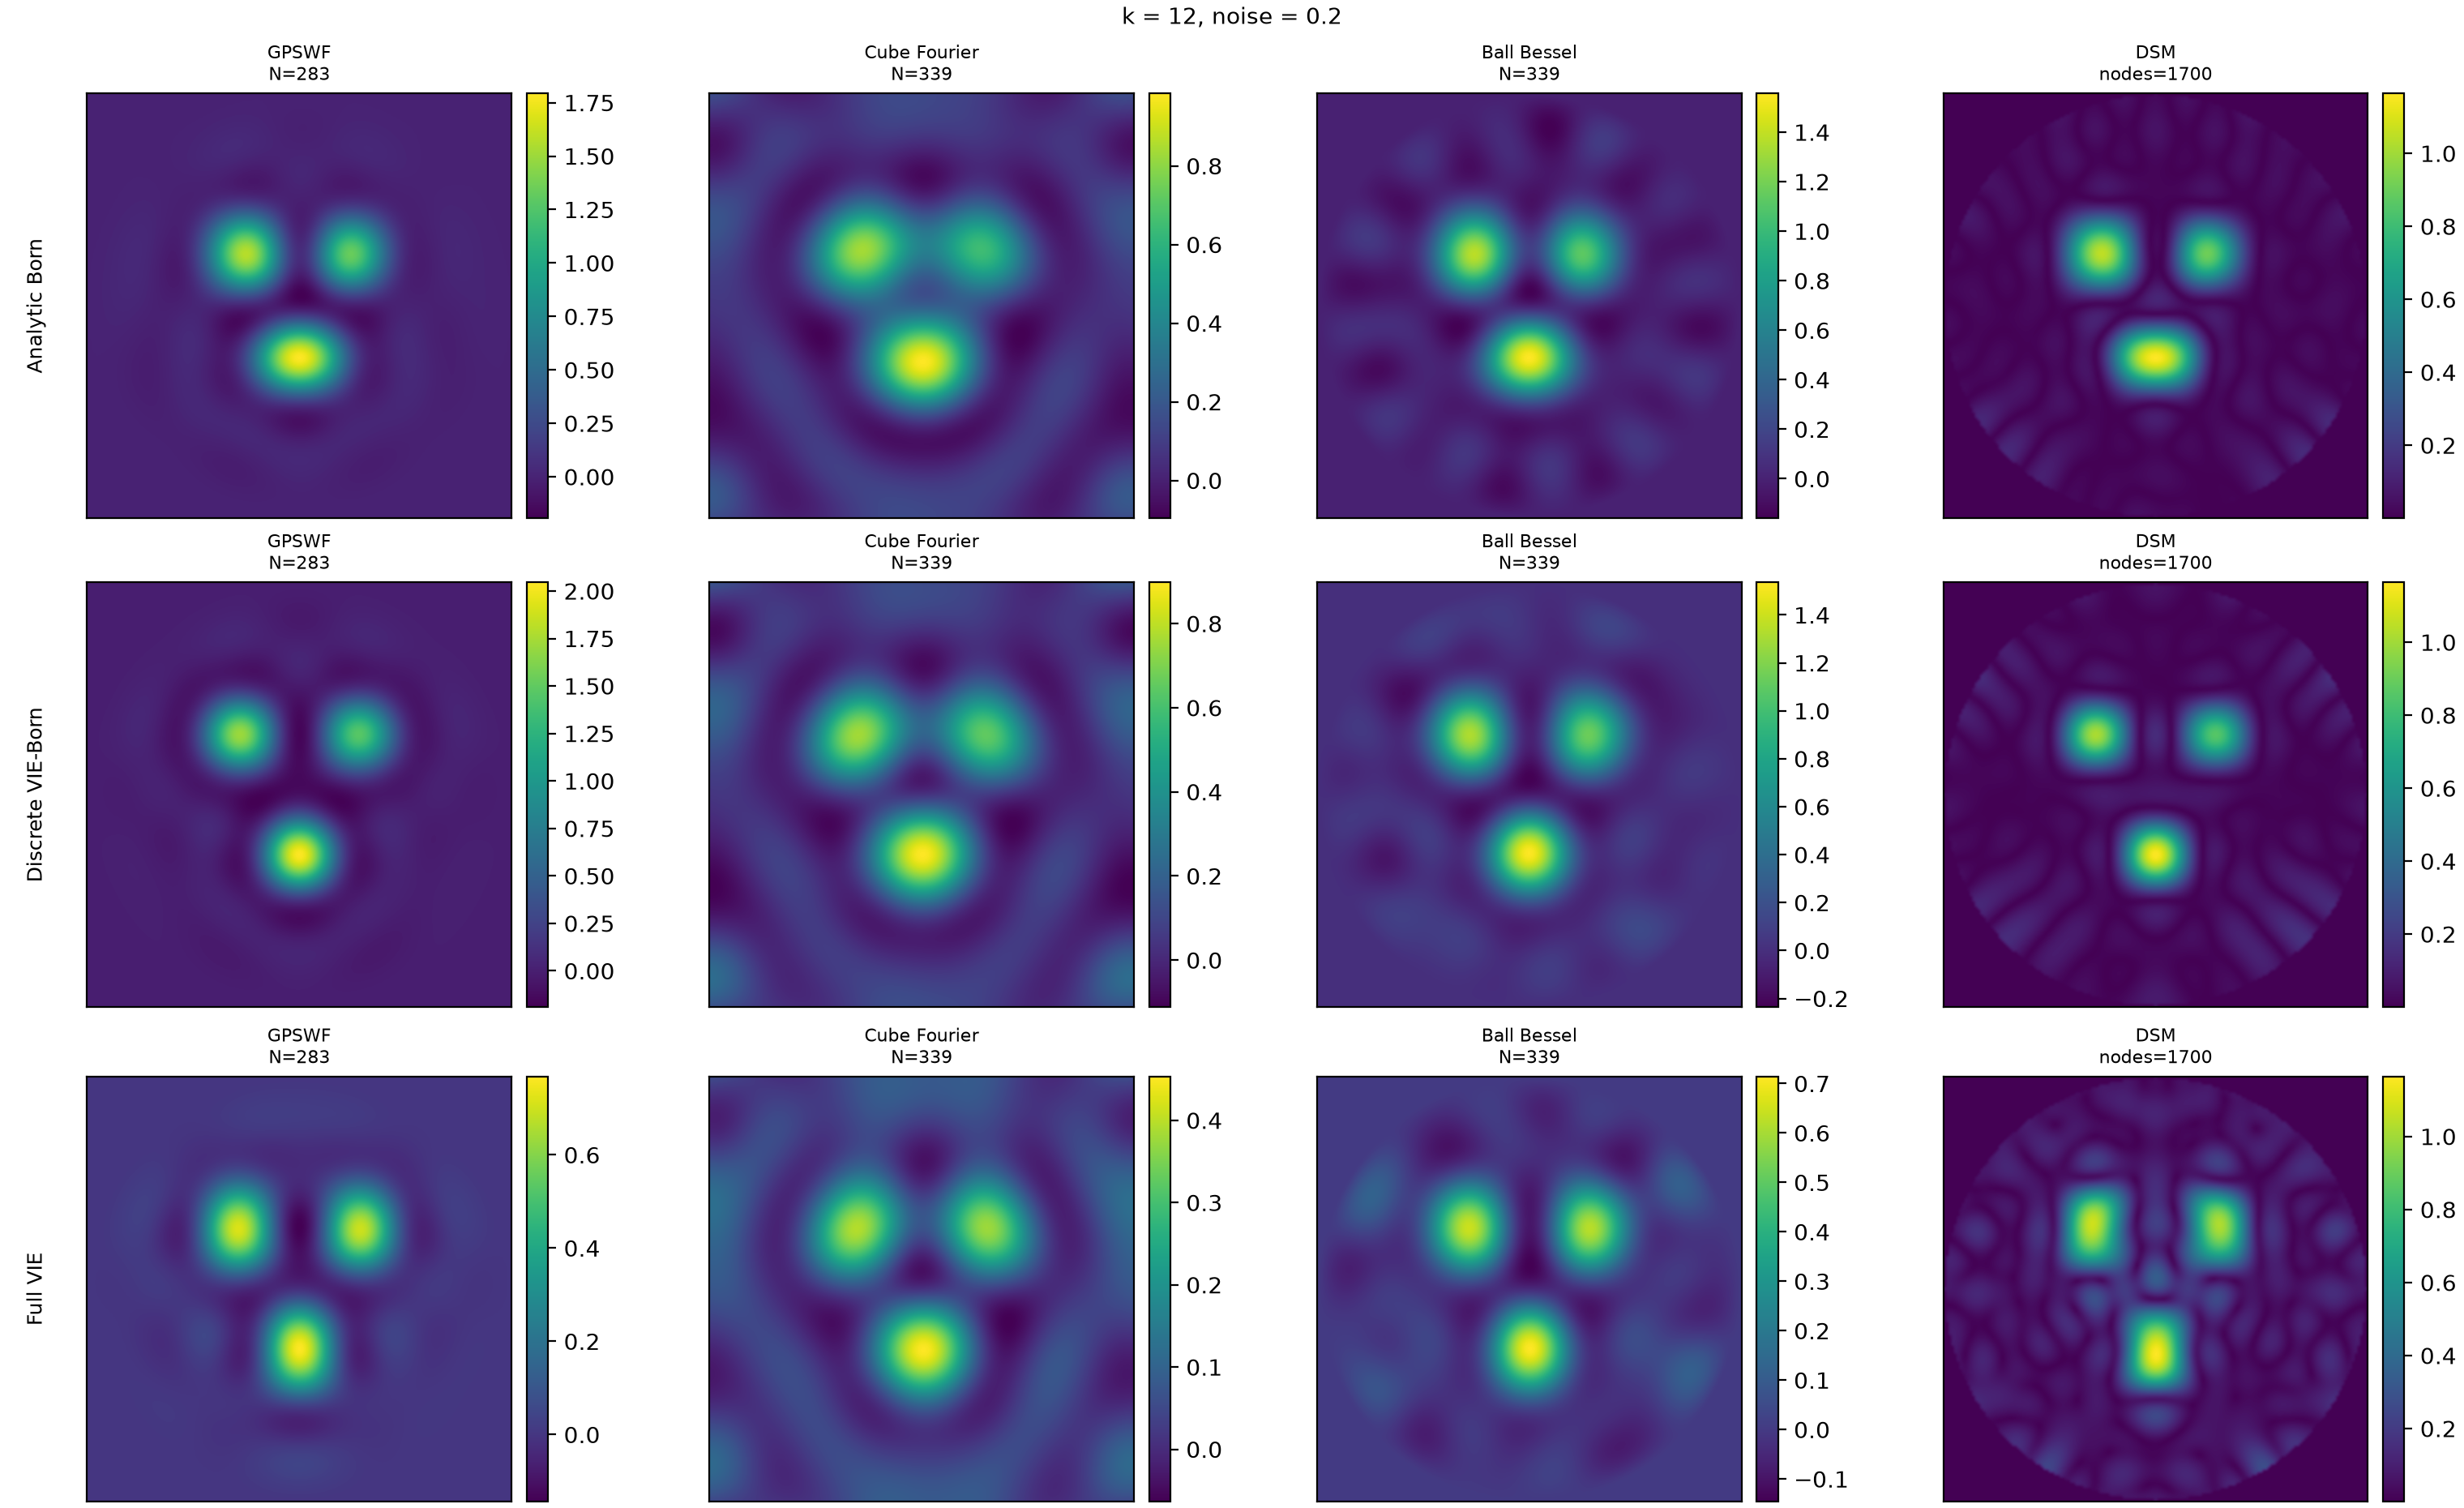
\includegraphics[width=\textwidth]
    {outputs/exp5/exp5_forward_comparison_individual_scale.png}
    \caption{GPSWF, cube Fourier, spherical Bessel, and DSM reconstructions
    from analytic Born, discrete VIE--Born, and Full VIE far-field data. Here
    $k=12$ and $\delta=0.2$. Every panel has an independent color scale.}
    \label{fig:maxwell-exp5-forward-sources}
\end{figure}

\subsection{Diagnostics and reproducibility}
\label{subsec:maxwell-gpswf-diagnostics}

Each experiment produces a scalar CSV diagnostic table, a compressed NPZ file
with detailed diagnostics, and diagnostic curves in addition to the
reconstruction figures. Table~\ref{tab:maxwell-output-files} summarizes their
roles.

\begin{table}[htbp]
    \centering
    \caption{Numerical experiment outputs.}
    \label{tab:maxwell-output-files}
    \begin{tabular}{ll}
        \toprule
        Output & Purpose\\
        \midrule
        \texttt{exp*\_*\_individual\_scale.png}
        & Individually scaled reconstruction panels\\
        \texttt{exp*\_diagnostics.csv} & Readable scalar diagnostics\\
        \texttt{exp*\_diagnostics\_detail.npz} & Compressed detailed diagnostics\\
        \texttt{exp*\_diagnostic\_curves.png} & Stability and leakage curves\\
        \texttt{exp3\_frequency\_dsm.png} & DSM frequency-comparison panels\\
        \texttt{exp3\_dsm\_diagnostics.csv} & DSM scalar diagnostics\\
        \texttt{exp1\_full\_vs\_born\_diagnostics.png}
        & Full VIE/Born radial diagnostic curves\\
        \texttt{exp1\_forward\_model\_diagnostics.csv}
        & Full VIE/Born scalar diagnostics\\
        \texttt{exp1\_forward\_model\_diagnostics\_detail.npz}
        & Full VIE/Born nodewise diagnostics\\
        \bottomrule
    \end{tabular}
\end{table}

The principal diagnostics include the retained mode count, the ratio of
quadrature nodes to retained modes, mean and maximum mock-node distances,
polarimetric singular values and condition numbers, the GPSWF Gram-matrix
condition number, the coefficient norm, the target-region amplitude, and the
95th percentile of the background amplitude. These quantities help isolate
errors originating from direction matching, polarimetric recovery, modal
projection, and image scaling.

Experiment 5 additionally records the relative far-field and recovered
$\widehat{\mathbf{Q}}$ differences with respect to analytic Born data. For the
Full VIE row it records the voxel and unknown counts, the number of unique
incident directions and right-hand sides, and sampled linear-system residuals.

Experiments 1--4 can be generated from the project root with
\begin{verbatim}
.venv/bin/python maxwell_gpswf/main.py \
    --mode all --out-dir outputs
\end{verbatim}
This command performs several dense Full VIE solves. In particular,
Experiment 1 uses $n_{\mathrm{axis}}=23$, corresponding to 19209 complex field
unknowns. Its dense matrix alone requires approximately 5.50 GiB, and LU
factorization requires additional memory. Experiment 2 and the $k=20$ case of
Experiment 3 use $n_{\mathrm{axis}}=19$, corresponding to 11085 unknowns and
approximately 1.83 GiB for the dense matrix. Formal runs should therefore be
executed only on a machine with sufficient memory. Quick-mode VIE grids are
intended only for code-path validation and not for physical accuracy claims.
Experiment 5 is a supplementary forward-source comparison and is deliberately
excluded from \texttt{--mode all}. It is run explicitly with
\begin{verbatim}
.venv/bin/python maxwell_gpswf/main.py \
    --mode exp5 --out-dir outputs
\end{verbatim}
